\documentclass[conference]{IEEEtran}
\IEEEoverridecommandlockouts
% The preceding line is only needed to identify funding in the first footnote. If that is unneeded, please comment it out.
\usepackage{cite}
\usepackage{amsmath,amssymb,amsfonts}
\usepackage{algorithmic}
\usepackage{graphicx}
\usepackage{textcomp}
\usepackage{xcolor}
\graphicspath{{resources/}}
\def\BibTeX{{\rm B\kern-.05em{\sc i\kern-.025em b}\kern-.08em
    T\kern-.1667em\lower.7ex\hbox{E}\kern-.125emX}}
\begin{document}

\title{Development of Code Execution Visualization as Interactive Learning Tool for Online Programming Learning Platform}

\author{
  \IEEEauthorblockN{Faris Rizki Ekananda}
  \IEEEauthorblockA{\textit{School of Electrical Engineering and Informatics} \\
    Institut Teknologi Bandung\\
    Bandung, Indonesia \\
    faris.ekananda20@gmail.com}
  \and
  \IEEEauthorblockN{Yudistira Asnar}
  \IEEEauthorblockA{\textit{School of Electrical Engineering and Informatics} \\
    Institut Teknologi Bandung\\
    Bandung, Indonesia \\
    yudis@itb.ac.id}
}

\maketitle

\begin{abstract}
  One of the challenges in learning programming for people who are new to programming is understanding how programs work. This is important because they still don't have an appropriate view of the program's working process, making it difficult for them to absorb the programming material they learn. This is made more difficult when learning is done online, because learning can take place asynchronously so that teachers must be able to ensure understanding can be achieved through learning materials without direct interaction.

  One way to improve understanding in learning is by creating an interactive learning environment (ILE). In some existing online programming learning platforms, interactive learning is done by working on problems using a Web IDE such as Sololearn, understanding concepts using interactive visual animations such as Brilliant, and presenting material using interactive storytelling on Progate. However, the use of visualization of the execution of the program as an ILE is still minimally used in programming learning classes, even though based on several literature studies it can improve the understanding of programming concepts because it can generate a concrete model of computer programming in novice students.

  In this paper, an ILE is built in the form of a code execution visualization tool that displays how the program works. This system is integrated with online programming classes on KodeBareng Web Platform so that it can be used in the learning process and practice problem solving. After conducting user experiments, the results show that this ILE is considered by users to be helpful in learning with an average score in the range of 4.231 and 4.385 on the likert scale, as well as increasing the average correct answer value on the questions tested with the most significant increase in concept understanding (using SOLO Level) in module 1 with a t value of 2.179 (\textit{p = 0.0147}) for students who have never learned programming before with an increase from an average SOLO Level score of 2.429 to 3.857 and in module 2 from an average SOLO Level of 3.333 to 3.6.
\end{abstract}

\begin{IEEEkeywords}
  programming learning, interactive learning, code execution visualization
\end{IEEEkeywords}

\section{Introduction}
The rapid development of digital technology opens up vast potential in online learning. With the help of the internet, learning can be done anywhere and anytime. Learning is no longer constrained by geographical and time boundaries so that there are more connections and interactions between teachers and students \cite{choy2004interactive,keengwe2010towards,psotka2012ile}.

However, the interaction between students and teachers in online learning cannot be equated with traditional learning. Interactions such as verbally asking students questions, encouraging students to solve problems in front of the class, and similar things cannot be done in asynchronous online learning because the interaction between the student and the teacher is not done directly.

One of the challenges experienced by people who are new to programming is the lack of understanding of what happens when a program executes a code \cite{mayer1981psychology, moons2013pilot}. This happens because they still don't have a proper idea of how a computer program works, which makes it difficult for them to grasp the fundamental and abstract concepts of learning programming for beginners. Online learning also makes this more difficult to overcome as there is less interaction between the student and the teacher during asynchronous learning, so the teacher has to use other tools to provide a concrete model to the student.

Currently, many programming learning platforms utilize interactive learning in the form of code exercises using Web IDEs, interactive visual animations, and interactive storytelling. However, these solutions cannot address the problems faced by students who have never learned programming before. An interactive environment that supports learning and practicing programming tasks is needed to solve these problems. Such a environment is aimed to improve concept understanding, make learning more interactive and facilitate the students during the learning process.

In this paper, we will focus on the development of a code execution visualization tool as an interactive learning environment that can support the conceptual understanding of how a program works for students who are new to programming. We will also observe the effect of the tool on the learning process of students.

\section{Literature Review}
\subsection{Interactive Learning}
Essentially, interactive learning is a method of learning that involves interaction between the student and the educational material, such as processing the material, completing tasks, or solving problems with the aim of building cognitive, affective, conative, and psychomotor learning outcomes. In short, there is a reciprocal action relationship between student and teacher which prevents learning from becoming passive. In the context of online learning, this can be achieved through digital technology that connects students and teachers.

The characteristics of interactive learning \cite{reeves2012interactive} are access to content, tasks, and problems by the students using digital technology such as computers with internet access. Furthermore, Reeves \cite{reeves2012interactive} explains that there are 2 approaches in the application of interactive learning, namely learning "through" interactive learning program and learning "with" interactive learning program. Learning "through" an interactive learning program means that the program provides the lesson in a variety of communication methods (focusing on the interactive delivery of the lesson) while learning "with" an interactive learning program utilizes cognitive tools that the student can use to build pieces of information into knowledge allowing the student to build their own familiar representational model of understanding. Learning "with" an interactive learning program is much more impactful as it facilitates critical thinking and higher-order thinking (HOT). The program or tool used in interactive learning is also referred to as an interactive learning environment (ILE).

\subsection{Interactive Learning Environment (ILE)}
There are various types of interactive learning environments that can support learning programming according to \cite{moons2013pilot}, such as \textit{microworlds} that use graphics like LOGO turtles or in the form of physical robots such as Lego Mindstorm Kit that use simplified programming languages, algorithm visualization tools to visualize the workflow of a specific algorithm, and code execution visualization tools that can display the flow of a program's work process when executed. Sites that offer online learning, such as \cite{sololearn2021media}, \cite{codesaya2021media}, \cite{brilliant2021media}, and learning portals of educational institutions or \textit{e-learning system} are also considered as ILEs using the first form of interactive learning approach which is " through" interactive learning because it is static.

One form of ILE used in learning programming is a web-based integrated development environment (IDE) (hereafter referred to as Web IDE), which allows programming learners to write code and run it. This is because Web IDEs allow users to directly implement code without having to do any setup first. The Web IDE can also ensure that the program execution environment will always be the same between one user and another, and increase portability because it can be done anytime and anywhere \cite{tran2013interactive}. These ILEs can be integrated with program execution visualization tools so as to improve learners' understanding of programming concepts \cite{moons2013pilot}. Such ILEs fall under the second interactive learning approach of "with" interactive learning as they provide tools that users can use to explore further. Examples of ILEs in the form of code execution visualizations can be seen in \ref{fig:pythontutor} and \ref{fig:evizor}

\begin{figure}[htbp]
  \centerline{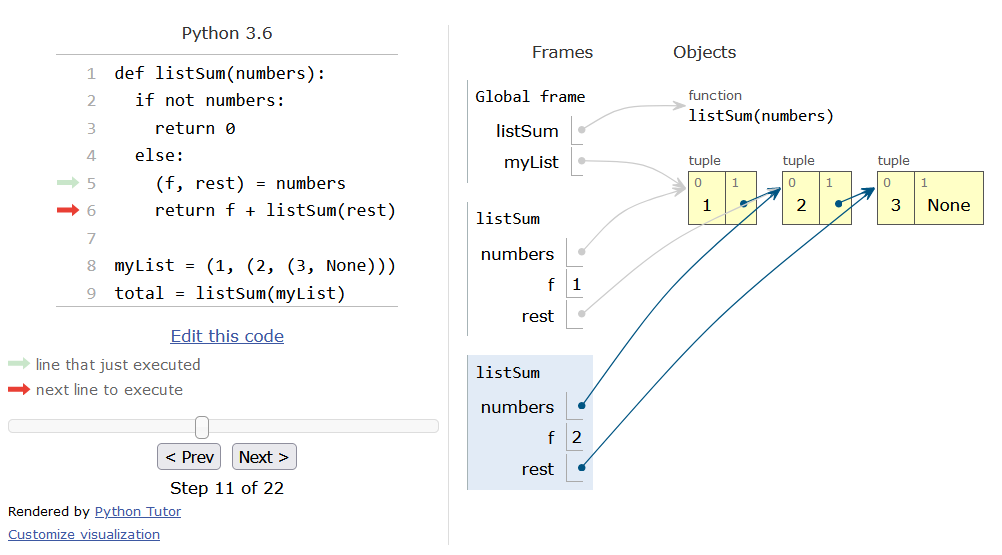
\includegraphics[width=\linewidth]{chapter2/pythontutor.png}}
  \caption{Code Execution Visualization in Python Tutor} \label{fig:pythontutor}
\end{figure}

\begin{figure}[htbp]
  \centerline{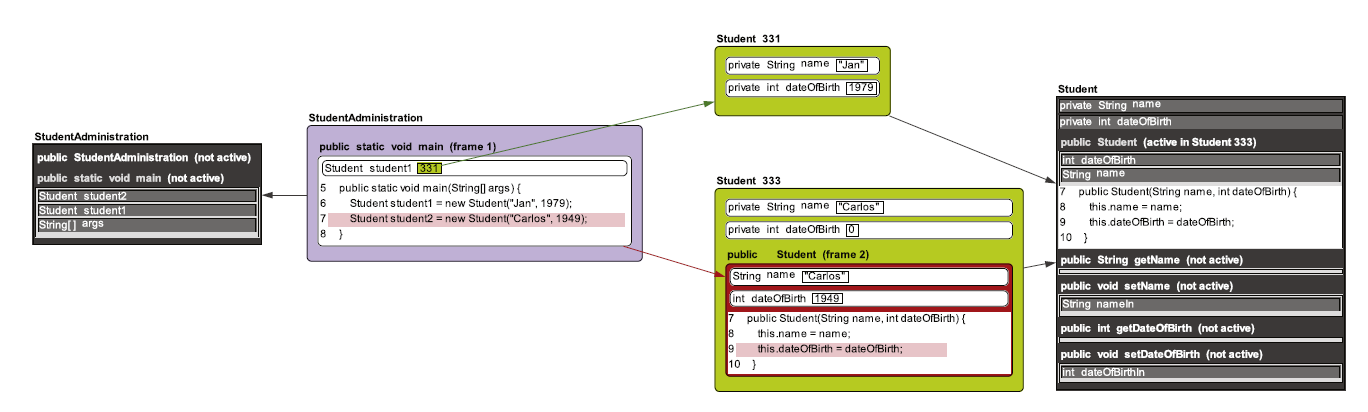
\includegraphics[width=\linewidth]{chapter2/evizor.png}}
  \caption{Code Execution Visualization in EVIZOR} \label{fig:evizor}
\end{figure}

\section{Related Works}

\section{Analysis and Design}
\subsection{Code Execution Visualization}
\subsection{Functional Requirement}
\subsection{Nonfunctional Requirement}
\subsection{Component Diagram}
\subsection{Stack Trace Processing}
\subsection{Visualizer}

\section{Implementation and Testing}
\subsection{Python Debugger}
\subsection{Implementation}
\subsection{Alpha Testing}
\subsection{User Experiment}
\subsection{Experiment Results}

\section{Conclusion and Future Work}

\bibliographystyle{IEEEtran}
\bibliography{IEEEabrv,IEEE}

\vspace{12pt}

\end{document}
